\taskpic{Человек, стоя на краю высокого обрыва, смотрит на ровное
  плоское дно котлована шириной $L$, заполненного водой глубины
  $h$. Высота обрыва $H$. Размеры котлована удовлетворяют неравенствам
  $L \gg H \gg h$. Показатель преломления воды равен $n$. Как зависит
  от расстояния до обрыва видимая глубина котлована?}{
  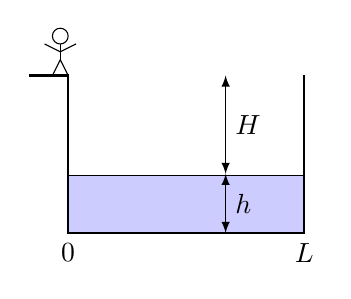
\begin{tikzpicture}[>=latex]
    \draw[fill=blue!20] (1,1) rectangle ++(3,0.73);
    \draw[thick] (0.5,3) -- ++(0.5,0) -- ++(0,-2) -- ++(3,0) --++(0,2);
    \draw[<->] (3,1) -- (3,1.75) node [midway,right] {$h$};
    \draw[<->] (3,1.75) -- (3,3) node [midway,right] {$H$};
    \draw (1,3) -- ++(-0.1,0.2) -- ++(-0.1,-0.2);
    \draw (0.9,3.2) -- ++(0,0.2);
    \draw (0.9,3.3) -- ++(0.2,0.1);
    \draw (0.9,3.3) -- ++(-0.2,0.1);
    \draw (0.9,3.5) circle (0.1);
    \draw (1,0.75) node {$0$};
    \draw (4,0.75) node {$L$};
  \end{tikzpicture}
  \vspace{0.5cm}
}
% Туймаада, 4.2